\documentclass{article}

\usepackage[%
    left=0.5in,%
    right=0.5in,%
    top=0.5in,%
    bottom=0.5in,%
]{geometry}%
\usepackage{minitoc}
\usepackage{multicol}
\usepackage{graphicx}
\usepackage{fixltx2e}
\usepackage{listings}
\usepackage{color}
\usepackage{hyperref}
    \hypersetup{ colorlinks = true, linkcolor = blue }
\usepackage{blindtext}
\definecolor{lightgray}{gray}{0.9}
\graphicspath{ {./} }

\newcommand{\inlinecode}[2]{\colorbox{lightgray}{\lstinline
[language=#1]$#2$}}
\newcommand{\worddef}[1]{\hyperref[sec:reference]{\textit{#1}}}

\begin{document}
	\section{Binary Search Trees}
	\begin{flushleft}
		A binary search tree is a binary tree storing keyvalue entries at its internal nodes and satisfying the following “search tree” property: Let $u, v$, and $w$ be any three nodes such that $u$ is in the \textbf{left} subtree of $v$ and $w$ is in the \textbf{right} subtree of $v$. Then we must have
		\[ key(u) < key(v) < key(w) \]
	\end{flushleft}	
	\begin{center}
		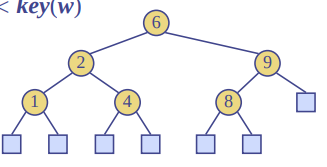
\includegraphics[scale=0.5]{binary_search_tree.png}
	\end{center}
	\begin{flushleft}
		External nodes \textbf{do not} store items and likely are \textbf{not actually implemented}, but are just \texttt{null} links from the parent
	\end{flushleft}
	
	\subsection{Search}
	\begin{flushleft}
	To search for key $k$, trace a downward path starting at the root. The next node visited depends on the outcome of the comparison of $k$ with the key of the current node. If we reach a leaf, the key is not found and we return \texttt{null}.
	\end{flushleft}
	\begin{center}
		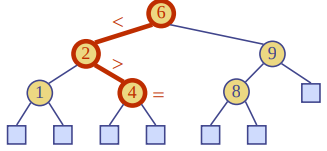
\includegraphics[scale=0.5]{binary_search_eg1.png}
	\end{center}
	
	\subsection{Insertion}	
	\begin{flushleft}
		Have to insert $k$ where a $get(k)$ would find it!. So natural that \texttt{insert(k,v)} starts with \texttt{get(k)}. We search for key $k$ (using \textit{TreeSearch}).
		\begin{itemize}
			\item  If $k$ is already in the tree then just replace the value
			\item Otherwise, $k$ is not already in the tree, and let $w$ be the leaf reached by the search
			\item We “insert $k$ at node $w$ and expand $w$ into an internal node”
		\end{itemize}
	\end{flushleft}	
	\begin{center}
		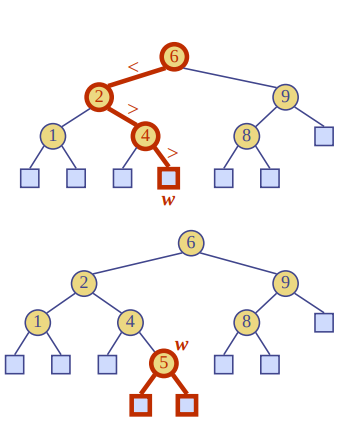
\includegraphics[scale=0.5]{binary_insert.png}
	\end{center}
	
	\subsection{Deletion}	
	\begin{itemize}
		\item As usual we start by trying to find(k)
		\item Four cases: (think of the externals as \texttt{null})
		\begin{itemize}
			\item k is not present. (Do nothing)
			\item n has no children (straightforward)
			\item n has one child,
			\item n has two children
		\end{itemize}
	\end{itemize}

	\subsubsection{Dealing with one child}
	\begin{multicols}{2}
		\begin{itemize}
			\item \texttt{remove(4)}
			\item Search for key 4. Let n be the node storing 4
			\item Node $n$ has a \texttt{null} (leaf) child $w$, and a real child 5
			\item We remove $n$ from the tree and connect 5 back to the parent of $n$
		\end{itemize}
		\begin{center}
			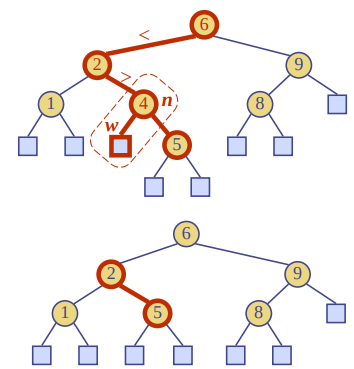
\includegraphics[scale=0.4]{binary_remove_1_child.png}		
		\end{center}
	\end{multicols}
	
	\subsubsection{Dealing with two children}
	\begin{multicols}{2}
	\begin{itemize}
		\item \texttt{remove(3)}
		\item As a sorted list, we would have \texttt{[1,2,3,5,6,8,9]}
		\item If we want to remove 3 then copy a key k’ that is adjacent to 3 on top of ‘3’ and then delete that key k’
		\item Options in this case are k’ being 2 or 5. We will focus on the nextKey, that is, ‘5
		\item The key node $n$ has two internal children
		\item Find the internal node $w$ that follows $n$ in an inorder traversal
		\item Copy \texttt{key(w)} into node $n$ 3
		\item Remove node $w$ and its left child $z$ (which must be a leaf) by means of same procedure as before for “one child”
	\end{itemize}
	\bigskip
	\begin{center}
		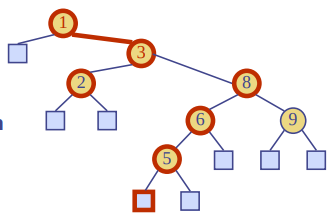
\includegraphics[scale=0.5]{binary_remove_2_children_base.png}
		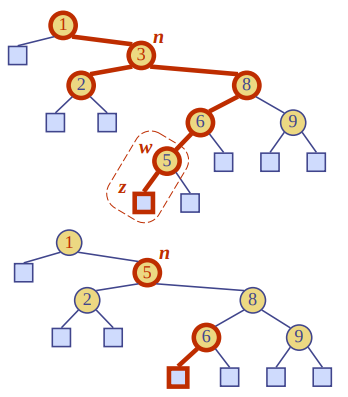
\includegraphics[scale=0.5]{binary_remove_2_children_flow.png}	
	\end{center}		
	\end{multicols}
	
	\subsection{Balanced Trees}
	\begin{flushleft}
		Binary search trees: if all levels filled, then search, insertion and deletion are \texttt{O(log N)}. However, performance may deteriorate to linear if nodes are inserted in order. (10 -> 11 -> 12)
	\end{flushleft}	
	
	\subsection{Performance}
	\begin{flushleft}
		Consider a binary search tree of height $h$ with $n$ items the space used is \texttt{O(n)}, methods find, \textbf{insert and remove} take \texttt{O(h)} time. The height $h$ is \texttt{O(n)} in the worst case and \texttt{O(log n)} in the best case. (Worst case: all nodes only have single child. Best case all nodes have two children)
	\end{flushleft}	

	\subsection{Self balancing}	
	\begin{flushleft}
		Constantly \textbf{re-structure} the trees: Keep the trees height \textbf{balanced} so that the height is logarithmic in the size Performance \textbf{always logarithmic}.
	\end{flushleft}	
	
	\subsubsection{Issues}
	\begin{flushleft}
		Suppose a very imbalanced search tree, there are always corresponding balanced search trees. Could make trees balanced using a \textit{total rebuild}. But would require $O(n)$, and so very \textbf{inefficient} compared to the desired $O(log \: n)$. Re-balancing needs to be $O(log \: n)$ or $O(height)$. Suggests re-balancing needs to just look at the path to some \textbf{recently changed node}, not the entire tree. A priori, it is not at all obvious that this is possible!
	\end{flushleft}

	\subsection{AVL trees}
	\begin{flushleft}
		\textbf{AVL} (Adelson-Velskii \& Landis) trees are \textit{binary search trees} where nodes also have additional information:
		\begin{itemize}
			\item The difference in \textbf{depth} between their right and left subtrees (\textit{balance factor}). 
			\item For each node, the \textit{balance factor} of that node is $height(right subtree) – height( left subtree )$ 
			\item In an AVL tree the balance of every node is allowed to be only \textbf{0,1 or -1}.
			\item AVL trees do \textbf{dynamic self-balancing} in $O(log \: n)$ time
		\end{itemize}
	\end{flushleft}	

	\subsection{Top down and bottom up insertion}	
	\begin{flushleft}
		\textbf{Top down} insertion algorithms make changes to the tree (necessary to keep the tree balanced) as they search for the place to insert the item. They make \textbf{one} pass through the tree. \textbf{Bottom up}: first insert the item, and then work \textbf{back} through the tree making changes. \textbf{Less efficient} because make \textbf{two passes} through the tree. (Need to find the item going from the top)
	\end{flushleft}	
	
	\pagebreak
	\section*{Reference section} \label{sec:reference}
	\begin{description}
		\item[load factor] \hfill \\ a measure of how full the hash table is allowed to get before its capacity is automatically increased.
	\end{description}
\end{document}
